\chapter{Acceso remoto y transferencia}\label{chap:3}
Esta práctica se centra en protocolos muy utilizados en la actualidad para
acceder a máquinas remotas y transferir archivos entre ellas. No se ha
realizado el apartado opcional de FTP{.}

Todo el código de esta práctica se encuentra dividido en carpetas según
el protocolo sobre el que se está trabajando. En cada carpeta se encuentran
los ficheros de cada ejercicio, con el nombre del ejercicio en cuestión.

\section{Acceso remoto}
\subsection{Telnet}
Para la realización de este apartado, se instala el servidor \Verb#telnetd# y su cliente y
se activa.

\begin{minipage}{\linewidth}
    \centering
    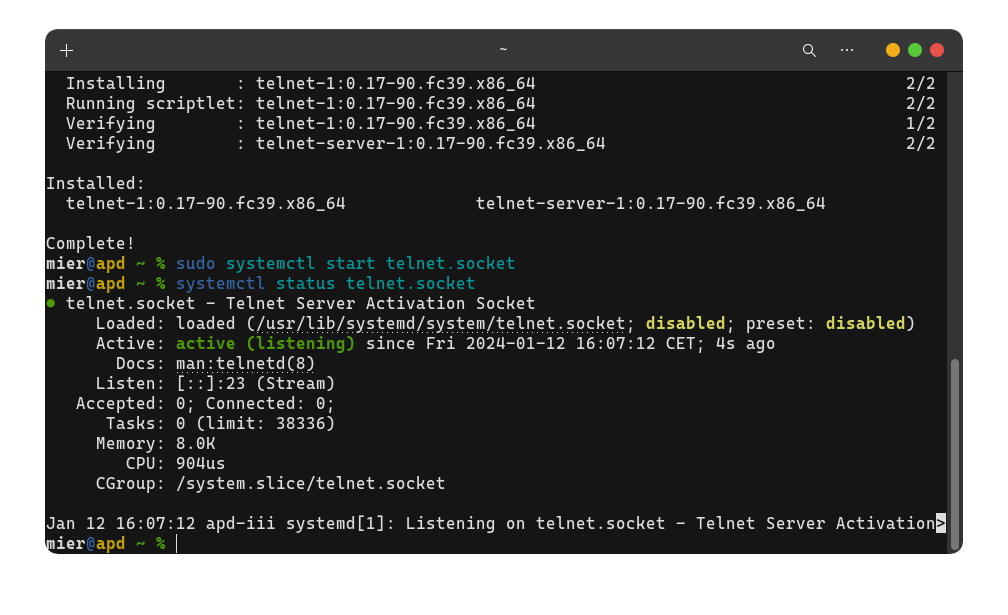
\includegraphics[width=\textwidth]{3/telnet0.png}
    \captionof{figure}{Instalación del servidor Telnet}\label{fig:3/1}
\end{minipage}

Como recuerda el enunciado, el servidor telnet no es seguro, por lo que se ha de desactivar
tras el desarrollo de los ejercicios.

Los siguientes ejercicios son solo pequeñas demostraciones prácticas sobre el protocolo, por
lo que no tienen grandes explicaciones.

\subsubsection{Ejercicio 1}
El ejercicio solicita que se escriba un programa \lstinline{telnet1_ejemplo.py}
que muestre por pantalla el resultado de ejecutar la orden \lstinline{ls} en el
directorio \Verb#/home#.

\begin{minipage}{\linewidth}
    \centering
    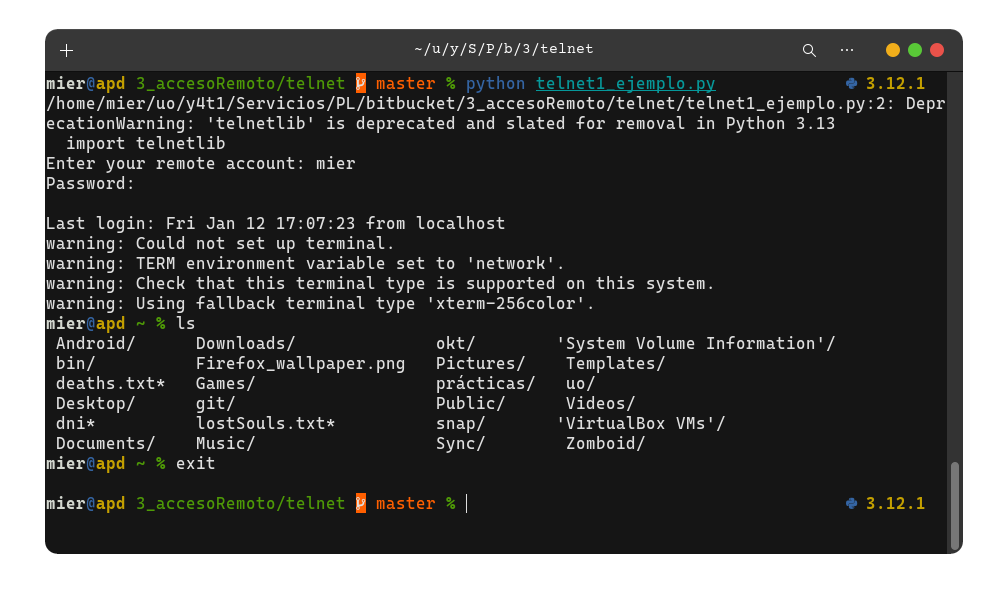
\includegraphics[width=\textwidth]{3/telnet1.png}
    \captionof{figure}{Ejercicio de ejemplo de Telnet}\label{fig:3/2}
\end{minipage}

El ejercicio solicita posteriormente que se mejore el programa \\
(\Verb#telnet1_ejemplo_mejorado.py#) para que omita el mensaje de bienvenida
del sistema.

\begin{minipage}{\linewidth}
    \centering
    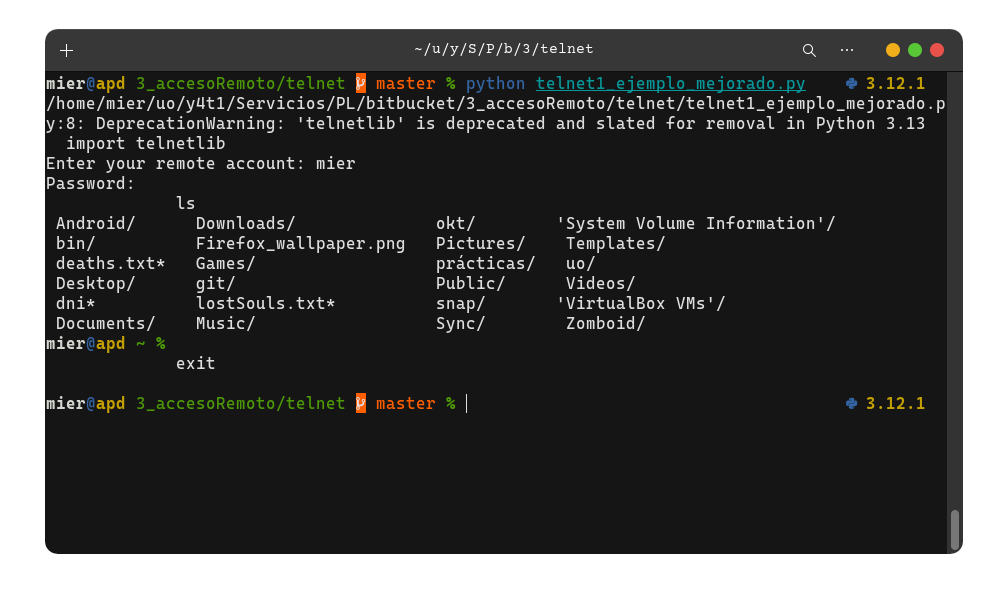
\includegraphics[width=\textwidth]{3/telnet2.png}
    \captionof{figure}{Ejercicio de ejemplo de Telnet mejorado}\label{fig:3/3}
\end{minipage}

\subsubsection{Ejercicio 2}

El ejercicio solicita escribir un programa \Verb#telnet2_lanza_servidor.py#
que lance un programa de la sesión \nameref{chap:1}.

Debido a que esta práctica se realiza en una máquina física Linux donde se acortan
los nombres de los procesos que se envían a través del comando \Verb#ps -ef#, el
ejercicio no funciona como esperado. El código que no funciona (validado por el
profesor) es el siguiente:

\begin{minipage}{\linewidth}
    \centering
    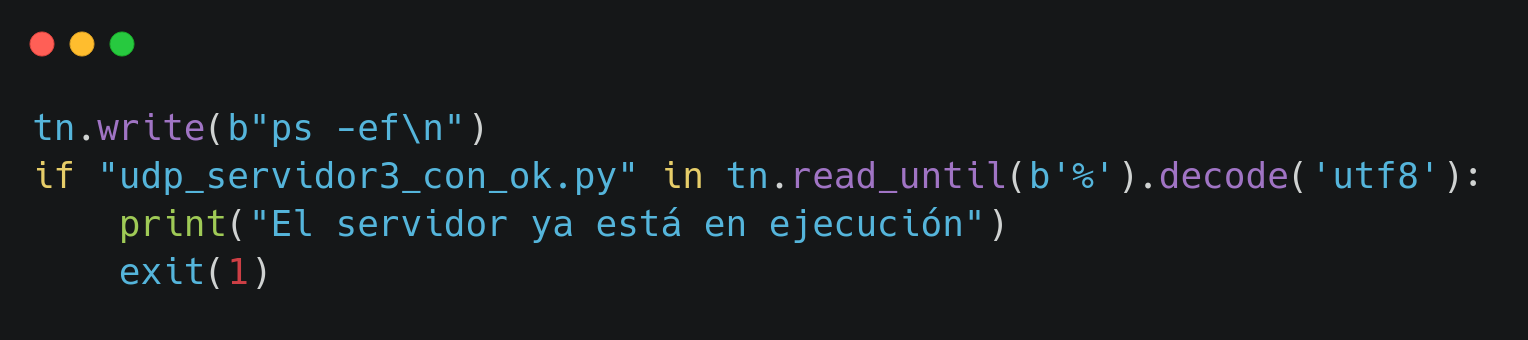
\includegraphics[width=\textwidth]{3/telnet_code1.png}
    \captionof{figure}{Código del ejercicio 2}\label{fig:3/4}
\end{minipage}

De todas formas, la esencia de la práctica es utilizar telnet para lanzar el servidor
UDP, por lo que se ignora la parte de la comprobación de procesos.

\begin{minipage}{\linewidth}
    \centering
    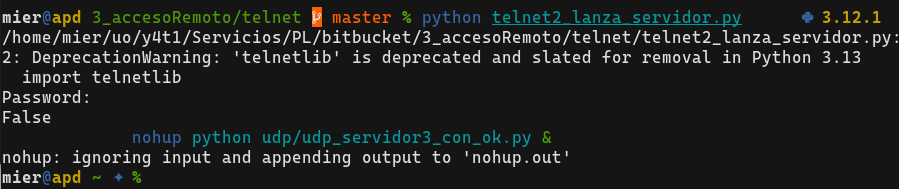
\includegraphics[width=\textwidth]{3/telnet3.png}
    \captionof{figure}{Telnet lanzando servidor UDP a través de nohup}\label{fig:3/5}
\end{minipage}

\subsection{SSH}
Puesto que el servidor SSH ya se encuentra instalado en la máquina, no es necesario
instalarlo. Todas las prácticas se realizan en plataformas Linux, por lo que se
utilizan las contrapartes de los programas de Windows que se utilizan en el enunciado.

\subsubsection{Ejercicio 3}
En este ejercicio, en lugar de PuTTY se utiliza el comand \Verb#ssh# directamente
para conectarse a un servidor remoto y verificar las huellas.

Para realizar este ejercicio, se utiliza un servidor externo que tenga SSH activado
y que nos permita obtener toda la información necesaria.

Al ejecutar el comando que nos otorga el fingerprint de la clave ED25519, obtenemos
el siguiente resultado: \Verb#SHA256:XWZjJrS...#. Al tratar de conectarnos al
servidor, verificamos que el fingerprint que nos muestra es el mismo que el que
nos ha dado el comando:
\begin{minipage}{\linewidth}
    \centering
    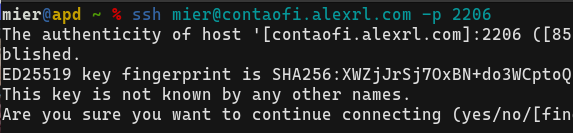
\includegraphics[width=\textwidth]{3/ssh1.png}
    \captionof{figure}{Fingerprint del servidor SSH}\label{fig:3/6}
\end{minipage}

\subsubsection{Ejercicio 4}
Para este ejercicio, en lugar de utilizar PuTTYgen, se utiliza el comando \Verb#ssh-keygen#
para generar la clave RSA{.}

\begin{minipage}{\linewidth}
    \centering
    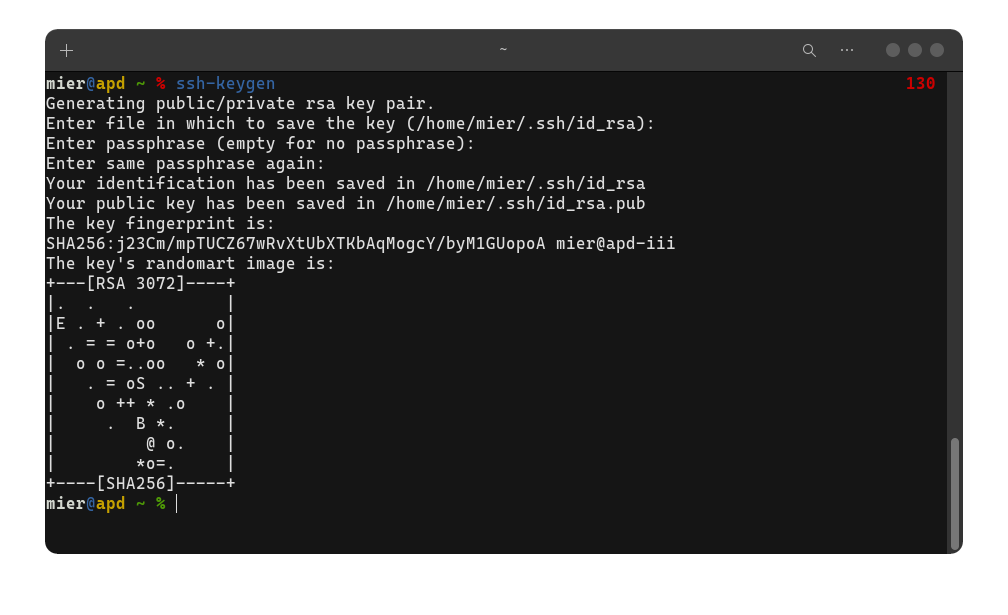
\includegraphics[width=\textwidth]{3/ssh2.png}
    \captionof{figure}{Generación de claves RSA}\label{fig:3/7}
\end{minipage}

El comando guarda automáticamente las claves en el directorio \Verb#~/.ssh# con los
nombres \Verb#id_rsa# y \Verb#id_rsa.pub#. Para poder utilizarlas, se copia la clave
pública al servidor remoto, en el fichero \Verb#~/.ssh/authorized_keys#.

\subsubsection{Ejercicio 5, 6}
Para utilizar las claves generadas en el ejercicio anterior, se ejecuta el comando
\Verb#ssh# junto con la opción \Verb#-i# para indicar la clave privada a utilizar.

\begin{minipage}{\linewidth}
    \centering
    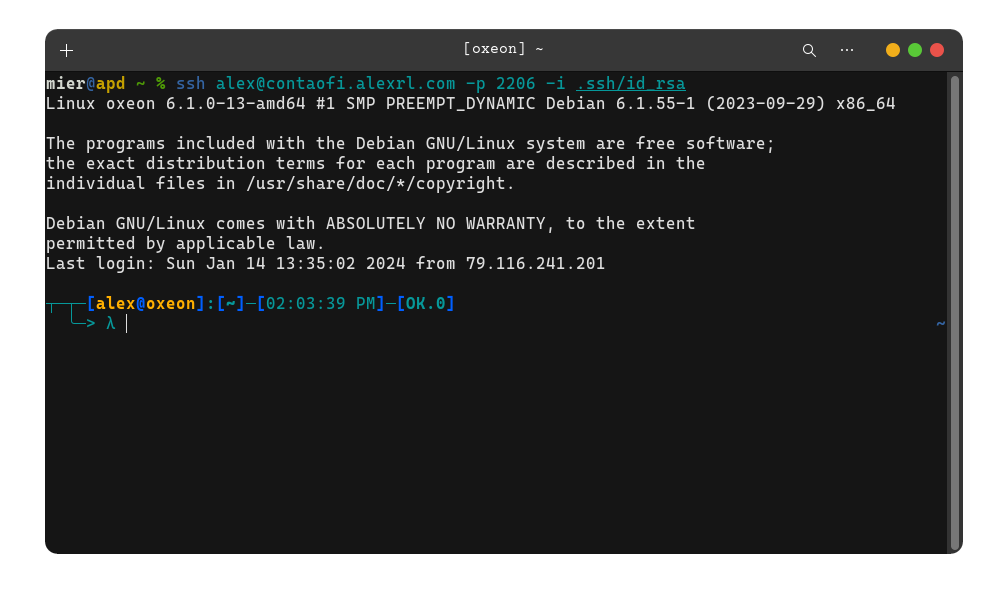
\includegraphics[width=\textwidth]{3/ssh3.png}
    \captionof{figure}{Conexión SSH con clave RSA}\label{fig:3/8}
\end{minipage}

\subsubsection{Ejercicio 7}
En lugar de \Verb#pageant#, se utiliza el comando \Verb#ssh-agent# para gestionar
las claves. Para añadir la clave privada al agente, se utiliza el comando
\Verb#ssh-add#. Para comprobar que la clave se ha añadido correctamente, se utiliza
el comando \Verb#ssh-add -l#.

\begin{minipage}{\linewidth}
    \centering
    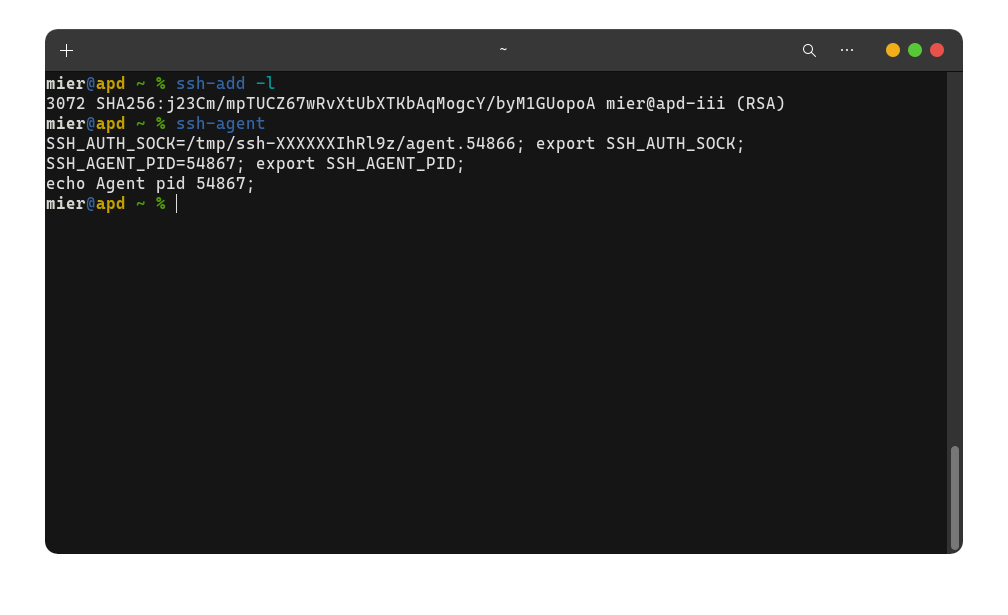
\includegraphics[width=\textwidth]{3/ssh4.png}
    \captionof{figure}{Gestión de claves con ssh-agent}\label{fig:3/9}
\end{minipage}

\begin{minipage}{\linewidth}
    \centering
    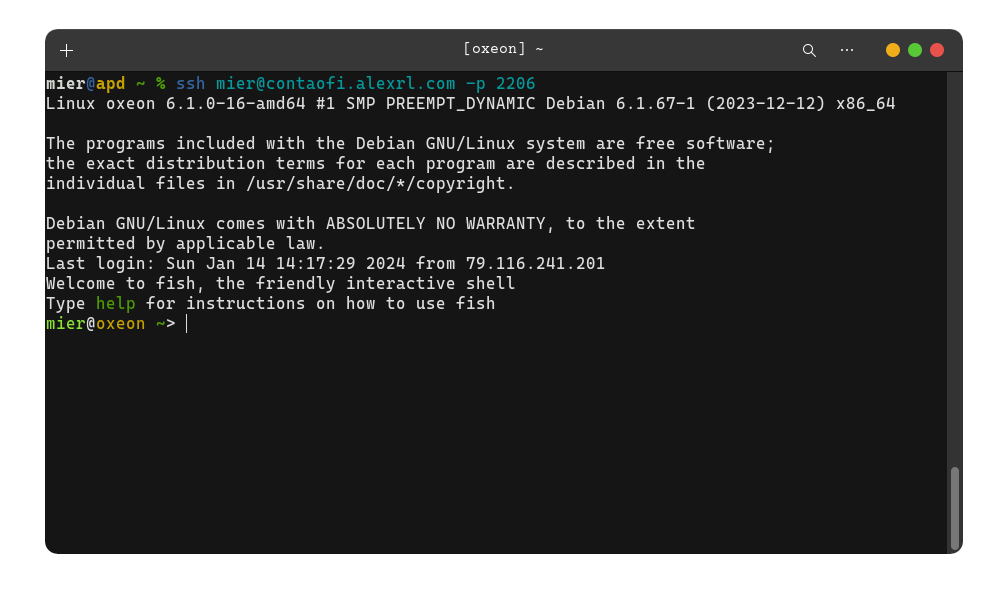
\includegraphics[width=\textwidth]{3/ssh5.png}
    \captionof{figure}{Demostración de autenticación mediante el agente}\label{fig:3/10}
\end{minipage}

\subsubsection{Ejercicio 8}
El ejercicio solicita que se modifique el programa \Verb#ssh_ejemplo_mal.py#
para que incluya la línea \Verb#client.set_missing_host_key_policy(paramiko.AutoAddPolicy())#
(resultando en el \Verb#ssh_ejemplo_inseguro.py#). Introducimos la línea en cuestión entre la
creación del cliente \Verb#paramiko# y la conexión con el servidor ssh para hacer que el cliente
acepte cualquier clave que le envíe el servidor.

Como dice el enunciado, la ejecución de esta ``solución'' resulta en un error.

\begin{minipage}{\linewidth}
    \centering
    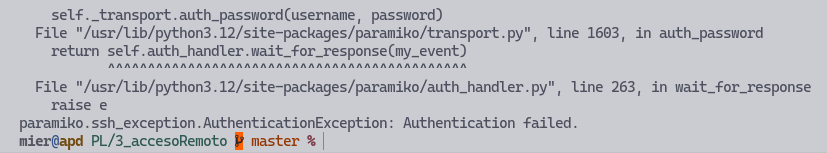
\includegraphics[width=\textwidth]{3/ssh6.png}
    \captionof{figure}{Error en la ejecución del ejemplo inseguro.}\label{fig:3/11}
\end{minipage}

La alternativa a esto es preguntarle al usuario directamente por la clave del servidor
y comprobar que es correcta antes de aceptarla.

\subsubsection{Ejercicio 9}
El ejercicio solicita que se modifique el programa \Verb#ssh_ejemplo_inseguro.py#
para que el cliente utilice la \Verb#WarningPolicy#.

Modificamos la política de la línea introducida en el ejercicio anterior y
obtenemos el fichero \Verb#ssh_ejemplo_inseguro2.py#. Este script sí que ejecuta
correctamente, pero muestra un mensaje de advertencia al usuario.

\begin{minipage}{\linewidth}
    \centering
    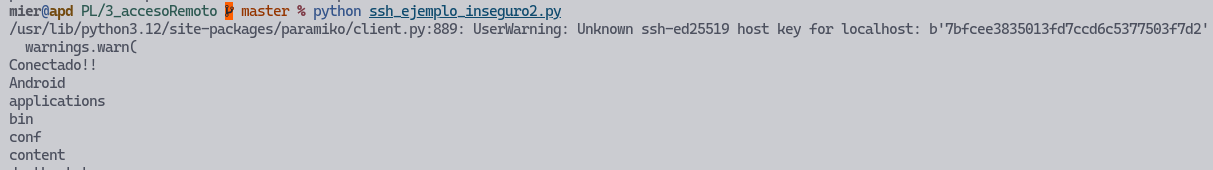
\includegraphics[width=\textwidth]{3/ssh7.png}
    \captionof{figure}{Ejecución del ejemplo inseguro 2.}\label{fig:3/12}
\end{minipage}

\subsubsection{Ejercicio 10}
El ejercicio solicita que se modifique el programa \Verb#ssh_ejemplo_inseguro2.py#,
eliminando la línea añadida previamente e insertando dos líneas nuevas para asegurar la conexión.

Para completar este ejercicio es necesario acceder al fichero \\
\Verb#/etc/ssh/ssh_host_ed25519_key.pub#, y añadir la clave pública del servidor,
que se pide por terminal al usuario.

\subsubsection{Ejercicio 11}

El ejercicio solicita que se modifique el programa \Verb#ssh_ejemplo_seguro.py#
para que sea posible conectarse al ordenador del compañero. Sigue la misma dinámica
de los ejercicios anteriores.

\section{Transferencia de archivos}
En esta sección se utilizan los protocolos \Verb#scp# y \Verb#sftp# para transferir
archivos entre máquinas remotas. Puesto que no se entra en muchos detalles en el
enunciado de la práctica, tampoco se comentan muchos detalles en esta memoria.

\subsubsection{Ejercicio 12}
Este ejercicio solicita que se utilice el programa \Verb#sftp# para conectarse a un
servidor remoto y listar los archivos que contiene.

\begin{minipage}{\linewidth}
    \centering
    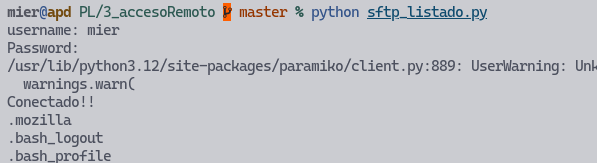
\includegraphics[width=\textwidth]{3/sftp1.png}
    \captionof{figure}{Listado de archivos con sftp}\label{fig:3/13}
\end{minipage}

\subsubsection{Ejercicio 13}
Este ejercicio solicita que se utilice el programa \Verb#sftp# para conectarse a un
servidor remoto y descargar todos los archivos (no directorios) del directorio \Verb#HOME#.

Se comenta el comando que descarga los ficheros para evitar tener que estar borrando y
descargando los ficheros cada vez que se ejecuta el script.

\begin{minipage}{\linewidth}
    \centering
    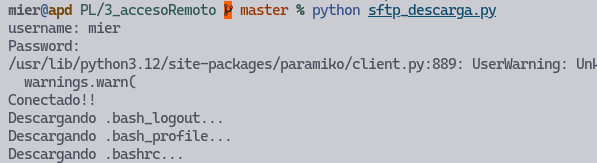
\includegraphics[width=\textwidth]{3/sftp2.png}
    \captionof{figure}{Descarga de archivos con sftp}\label{fig:3/14}
\end{minipage}

\section{Conclusiones}

\begin{center}
	\begin{tabular}{|c|c|}
		\hline
		\textbf{Autor} & \textbf{Porcentaje} \\
		\hline
		\hline
		\authorOne & 0\% \\
		\authorTwo & 1000\% \\
		\hline
	\end{tabular}
\end{center}
